% Options for packages loaded elsewhere
% Options for packages loaded elsewhere
\PassOptionsToPackage{unicode}{hyperref}
\PassOptionsToPackage{hyphens}{url}
\PassOptionsToPackage{dvipsnames,svgnames,x11names}{xcolor}
%
\documentclass[
  letterpaper,
  DIV=11,
  numbers=noendperiod,
  oneside]{scrartcl}
\usepackage{xcolor}
\usepackage[left=1in,marginparwidth=2.0666666666667in,textwidth=4.1333333333333in,marginparsep=0.3in]{geometry}
\usepackage{amsmath,amssymb}
\setcounter{secnumdepth}{-\maxdimen} % remove section numbering
\usepackage{iftex}
\ifPDFTeX
  \usepackage[T1]{fontenc}
  \usepackage[utf8]{inputenc}
  \usepackage{textcomp} % provide euro and other symbols
\else % if luatex or xetex
  \usepackage{unicode-math} % this also loads fontspec
  \defaultfontfeatures{Scale=MatchLowercase}
  \defaultfontfeatures[\rmfamily]{Ligatures=TeX,Scale=1}
\fi
\usepackage{lmodern}
\ifPDFTeX\else
  % xetex/luatex font selection
\fi
% Use upquote if available, for straight quotes in verbatim environments
\IfFileExists{upquote.sty}{\usepackage{upquote}}{}
\IfFileExists{microtype.sty}{% use microtype if available
  \usepackage[]{microtype}
  \UseMicrotypeSet[protrusion]{basicmath} % disable protrusion for tt fonts
}{}
\makeatletter
\@ifundefined{KOMAClassName}{% if non-KOMA class
  \IfFileExists{parskip.sty}{%
    \usepackage{parskip}
  }{% else
    \setlength{\parindent}{0pt}
    \setlength{\parskip}{6pt plus 2pt minus 1pt}}
}{% if KOMA class
  \KOMAoptions{parskip=half}}
\makeatother
% Make \paragraph and \subparagraph free-standing
\makeatletter
\ifx\paragraph\undefined\else
  \let\oldparagraph\paragraph
  \renewcommand{\paragraph}{
    \@ifstar
      \xxxParagraphStar
      \xxxParagraphNoStar
  }
  \newcommand{\xxxParagraphStar}[1]{\oldparagraph*{#1}\mbox{}}
  \newcommand{\xxxParagraphNoStar}[1]{\oldparagraph{#1}\mbox{}}
\fi
\ifx\subparagraph\undefined\else
  \let\oldsubparagraph\subparagraph
  \renewcommand{\subparagraph}{
    \@ifstar
      \xxxSubParagraphStar
      \xxxSubParagraphNoStar
  }
  \newcommand{\xxxSubParagraphStar}[1]{\oldsubparagraph*{#1}\mbox{}}
  \newcommand{\xxxSubParagraphNoStar}[1]{\oldsubparagraph{#1}\mbox{}}
\fi
\makeatother


\usepackage{longtable,booktabs,array}
\newcounter{none} % for unnumbered tables
\usepackage{calc} % for calculating minipage widths
% Correct order of tables after \paragraph or \subparagraph
\usepackage{etoolbox}
\makeatletter
\patchcmd\longtable{\par}{\if@noskipsec\mbox{}\fi\par}{}{}
\makeatother
% Allow footnotes in longtable head/foot
\IfFileExists{footnotehyper.sty}{\usepackage{footnotehyper}}{\usepackage{footnote}}
\makesavenoteenv{longtable}
\usepackage{graphicx}
\makeatletter
\newsavebox\pandoc@box
\newcommand*\pandocbounded[1]{% scales image to fit in text height/width
  \sbox\pandoc@box{#1}%
  \Gscale@div\@tempa{\textheight}{\dimexpr\ht\pandoc@box+\dp\pandoc@box\relax}%
  \Gscale@div\@tempb{\linewidth}{\wd\pandoc@box}%
  \ifdim\@tempb\p@<\@tempa\p@\let\@tempa\@tempb\fi% select the smaller of both
  \ifdim\@tempa\p@<\p@\scalebox{\@tempa}{\usebox\pandoc@box}%
  \else\usebox{\pandoc@box}%
  \fi%
}
% Set default figure placement to htbp
\def\fps@figure{htbp}
\makeatother

\ifLuaTeX
  \usepackage{luacolor}
  \usepackage[soul]{lua-ul}
\else
  \usepackage{soul}
\fi

% definitions for citeproc citations
\NewDocumentCommand\citeproctext{}{}
\NewDocumentCommand\citeproc{mm}{%
  \begingroup\def\citeproctext{#2}\cite{#1}\endgroup}
\makeatletter
 % allow citations to break across lines
 \let\@cite@ofmt\@firstofone
 % avoid brackets around text for \cite:
 \def\@biblabel#1{}
 \def\@cite#1#2{{#1\if@tempswa , #2\fi}}
\makeatother
\newlength{\cslhangindent}
\setlength{\cslhangindent}{1.5em}
\newlength{\csllabelwidth}
\setlength{\csllabelwidth}{3em}
\newenvironment{CSLReferences}[2] % #1 hanging-indent, #2 entry-spacing
 {\begin{list}{}{%
  \setlength{\itemindent}{0pt}
  \setlength{\leftmargin}{0pt}
  \setlength{\parsep}{0pt}
  % turn on hanging indent if param 1 is 1
  \ifodd #1
   \setlength{\leftmargin}{\cslhangindent}
   \setlength{\itemindent}{-1\cslhangindent}
  \fi
  % set entry spacing
  \setlength{\itemsep}{#2\baselineskip}}}
 {\end{list}}
\usepackage{calc}
\newcommand{\CSLBlock}[1]{\hfill\break\parbox[t]{\linewidth}{\strut\ignorespaces#1\strut}}
\newcommand{\CSLLeftMargin}[1]{\parbox[t]{\csllabelwidth}{\strut#1\strut}}
\newcommand{\CSLRightInline}[1]{\parbox[t]{\linewidth - \csllabelwidth}{\strut#1\strut}}
\newcommand{\CSLIndent}[1]{\hspace{\cslhangindent}#1}



\setlength{\emergencystretch}{3em} % prevent overfull lines

\providecommand{\tightlist}{%
  \setlength{\itemsep}{0pt}\setlength{\parskip}{0pt}}



 


\KOMAoption{captions}{tableheading}
\makeatletter
\@ifpackageloaded{tcolorbox}{}{\usepackage[skins,breakable]{tcolorbox}}
\@ifpackageloaded{fontawesome5}{}{\usepackage{fontawesome5}}
\definecolor{quarto-callout-color}{HTML}{909090}
\definecolor{quarto-callout-note-color}{HTML}{0758E5}
\definecolor{quarto-callout-important-color}{HTML}{CC1914}
\definecolor{quarto-callout-warning-color}{HTML}{EB9113}
\definecolor{quarto-callout-tip-color}{HTML}{00A047}
\definecolor{quarto-callout-caution-color}{HTML}{FC5300}
\definecolor{quarto-callout-color-frame}{HTML}{acacac}
\definecolor{quarto-callout-note-color-frame}{HTML}{4582ec}
\definecolor{quarto-callout-important-color-frame}{HTML}{d9534f}
\definecolor{quarto-callout-warning-color-frame}{HTML}{f0ad4e}
\definecolor{quarto-callout-tip-color-frame}{HTML}{02b875}
\definecolor{quarto-callout-caution-color-frame}{HTML}{fd7e14}
\makeatother
\makeatletter
\@ifpackageloaded{caption}{}{\usepackage{caption}}
\AtBeginDocument{%
\ifdefined\contentsname
  \renewcommand*\contentsname{Table of contents}
\else
  \newcommand\contentsname{Table of contents}
\fi
\ifdefined\listfigurename
  \renewcommand*\listfigurename{List of Figures}
\else
  \newcommand\listfigurename{List of Figures}
\fi
\ifdefined\listtablename
  \renewcommand*\listtablename{List of Tables}
\else
  \newcommand\listtablename{List of Tables}
\fi
\ifdefined\figurename
  \renewcommand*\figurename{Figure}
\else
  \newcommand\figurename{Figure}
\fi
\ifdefined\tablename
  \renewcommand*\tablename{Table}
\else
  \newcommand\tablename{Table}
\fi
}
\@ifpackageloaded{float}{}{\usepackage{float}}
\floatstyle{ruled}
\@ifundefined{c@chapter}{\newfloat{codelisting}{h}{lop}}{\newfloat{codelisting}{h}{lop}[chapter]}
\floatname{codelisting}{Listing}
\newcommand*\listoflistings{\listof{codelisting}{List of Listings}}
\makeatother
\makeatletter
\makeatother
\makeatletter
\@ifpackageloaded{caption}{}{\usepackage{caption}}
\@ifpackageloaded{subcaption}{}{\usepackage{subcaption}}
\makeatother
\makeatletter
\@ifpackageloaded{sidenotes}{}{\usepackage{sidenotes}}
\@ifpackageloaded{marginnote}{}{\usepackage{marginnote}}
\makeatother
\makeatletter
\@ifpackageloaded{algorithm}{}{\usepackage{algorithm}}
\makeatother
\makeatletter
\@ifpackageloaded{algpseudocode}{}{\usepackage{algpseudocode}}
\makeatother
\makeatletter
\@ifpackageloaded{caption}{}{\usepackage{caption}}
\makeatother
    \makeatletter
    \newcommand\fs@nocaption{
      \def\@fs@cfont{\bfseries}
      \let\@fs@capt\floatc@plain
      \def\@fs@pre{}%
      \def\@fs@post{\kern2pt\hrule}%
      \def\@fs@mid{\hrule\kern2pt}%
      \let\@fs@iftopcapt\iftrue}
    \makeatother
  
\captionsetup[algorithm]{justification=raggedright}
\usepackage{bookmark}
\IfFileExists{xurl.sty}{\usepackage{xurl}}{} % add URL line breaks if available
\urlstyle{same}
\hypersetup{
  pdftitle={Training Classifiers with Natural Language Explanations},
  pdfkeywords={BabbleLabble, Feature Engineering, Function
Learning, Explanation-Based Learning, Semantic Parsing, Aggregation},
  colorlinks=true,
  linkcolor={blue},
  filecolor={Maroon},
  citecolor={Blue},
  urlcolor={Blue},
  pdfcreator={LaTeX via pandoc}}


\title{Training Classifiers with Natural Language Explanations}
\usepackage{etoolbox}
\makeatletter
\providecommand{\subtitle}[1]{% add subtitle to \maketitle
  \apptocmd{\@title}{\par {\large #1 \par}}{}{}
}
\makeatother
\subtitle{Paper Review}
\author{}
\date{Tuesday, January 28, 2025}
\begin{document}
\maketitle

\algrenewcommand{\algorithmiccomment}[1]{\hskip3em$\rightarrow$ #1}

\floatname{algorithm}{Algorithm}


\begin{figure}[H]

{\centering \pandocbounded{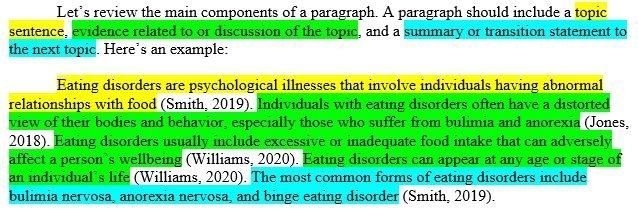
\includegraphics[keepaspectratio]{cover.jpg}}

}

\caption{litrature review}

\end{figure}%

\begin{marginfigure}

\centering{

\url{https://youtu.be/YBeAX-deMDg}

}

\caption{\label{fig-vid01}Babble Labble: Learning From Natural Language
Explanations (NIPS 2017 Demo)}

\end{marginfigure}%

\begin{marginfigure}

\centering{

\url{https://youtu.be/4cgvIh9DUrg}

}

\caption{\label{fig-vid01}Braden Hancock - Training Classifiers with
Natural Language Explanations}

\end{marginfigure}%

In (Hancock et al. 2018) the authors consider how to learn labeling
functions from natural language explanations. Such explanations can come
from a data labeler on Amazon mechnical Turk, a domain expert and
perhaps from an LLM. Labeling function capture a heuristic for labeling
data. The author ties it up with some work on \textbf{data programming}
which lead to \href{https://www.snorkel.org/}{snorkel} another data
labeling tool. This paper isn't about RL at all. It is interesting for a
number if reasons.

The hook for me was its approach to aggregation. Since Scott E. Page
pointed out the challenges of aggregation in his book
\href{https://www.amazon.com/Difference-Diversity-Creates-Complexity-Scott/dp/0691138540}{The
Difference} I have been considering how it manifests in many forms -
particularly in language emergence.

The chart I saw for the presentation was extremely similar to another
chart I had seen in a paper on emergent languages. It looked like this
paper was solving an aggregation problem I had been considering in
emergent languages. It turned out to be a coincidence. These are
different problems, and they aggregation is for different things. And
yet there still seems to be an underlying similarity.

\begin{enumerate}
\def\labelenumi{\arabic{enumi}.}
\tightlist
\item
  Another aspect of the paper is the approach to aggregating weak noisy
  classifier into a more powerful one. This aspect seems to also have
  merits for agents that are learning to discriminate together with
  learning a language. It is interesting that both Yoav Golderg and the
  Authors of this paper think that parsing accuracy is not that
  important since the parsers are good enough and their system is built
  to be robust to errors.
\item
  It uses \textbf{semantic parsers} to convert natural language
  explanations into labeling functions. Back in 2019
  \href{https://youtu.be/e12danHhlic?t=853}{Yoav Goldberg} i suggested
  in that too often NLP devs use RegEx instead of a more robust approach
  based on syntax trees that can be constructed thanks to Spacy. I think
  semantic parsers are perhaps one step further where we take the parse
  tree and convert it to a program.
\item
  Seems similar to the approach of I saw in
  \href{https://explosion.ai/blog/prodigy-annotation-tool-active-learning}{Prodigy}
  by spacey core developer \href{https://ines.io/}{Ines Montani} and
  others.
\item
  It implements
  \href{https://orenbochman.github.io/blog/notes/cognitivie-ai-cs7637/17-explanation-based-learning/17-explanation-based-learning.html}{Explanation-Based
  Learning} from Cognitive AI (CS7637) course.
\end{enumerate}

\begin{tcolorbox}[enhanced jigsaw, arc=.35mm, bottomrule=.15mm, bottomtitle=1mm, breakable, colback=white, colbacktitle=quarto-callout-tip-color!10!white, colframe=quarto-callout-tip-color-frame, coltitle=black, left=2mm, leftrule=.75mm, opacityback=0, opacitybacktitle=0.6, rightrule=.15mm, title=\textcolor{quarto-callout-tip-color}{\faLightbulb}\hspace{0.5em}{TL;DR - The paper}, titlerule=0mm, toprule=.15mm, toptitle=1mm]

\begin{figure}[H]

{\centering \pandocbounded{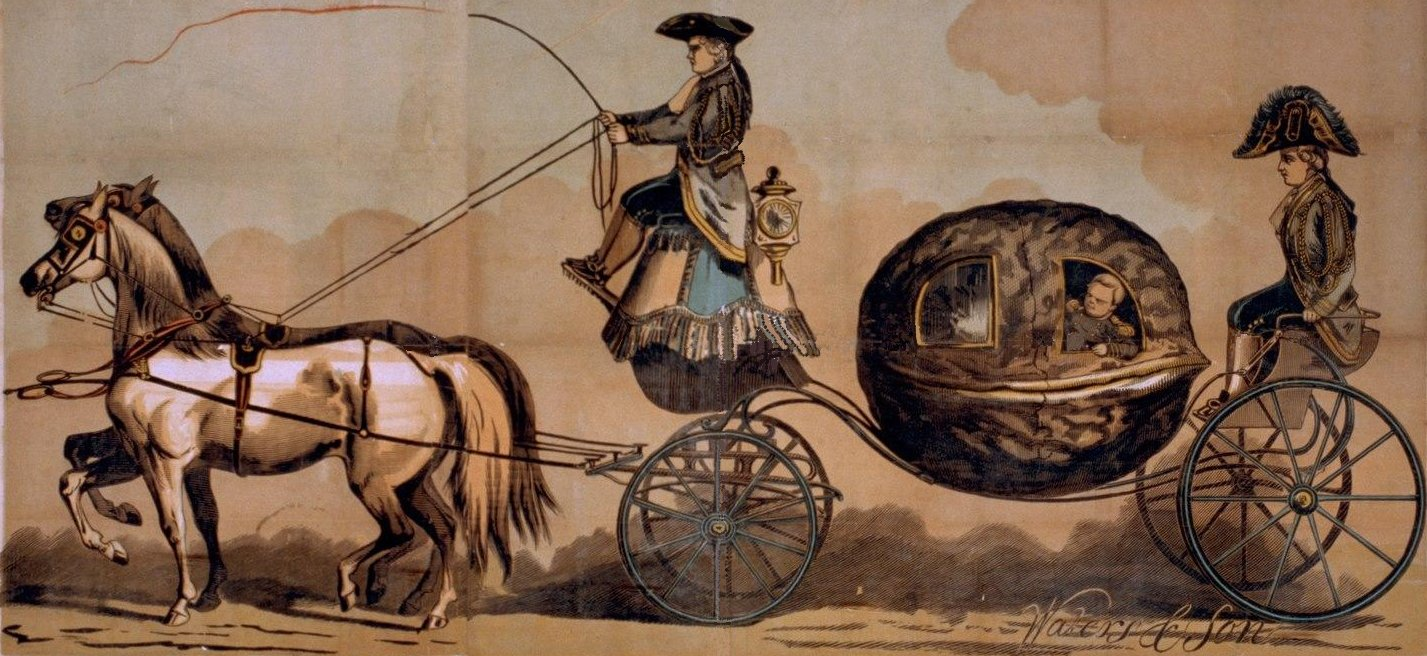
\includegraphics[keepaspectratio]{../img/in_a_nutshell.jpg}}

}

\caption{The paper in a nutshell}

\end{figure}%

BabbleLabble is a framework for training classifiers in which annotators
provide natural language explanations for labeling decisions. These
explanations are parsed into labeling functions that generate noisy
labels for unlabeled data. The framework consists of a semantic parser,
filter bank, and label aggregator. Experiments on relation extraction
tasks show that users can train classifiers 5-100× faster by providing
explanations instead of just labels. The filter bank effectively removes
incorrect labeling functions, and the label aggregator combines labels
into probabilistic labels for training a discriminative model. The noisy
labels provide weak supervision that promotes generalization.

\end{tcolorbox}

\begin{marginfigure}

\centering{

\begin{figure}
\centering
\pandocbounded{
\includegraphics[keepaspectratio,alt={BabbleLabble UI}]{fig-01.png}}
\caption{BabbleLabble UI}
\end{figure}

}

\caption{\label{fig-01}In BabbleLabble, the user provides a natural
language explanation for each labeling decision. These explanations are
parsed into labeling functions that convert unlabeled data into a large
labeled dataset for training a classifier.}

\end{marginfigure}%

\subsection{Abstract}\label{abstract}

\begin{quote}
Training accurate classifiers requires many labels, but each label
provides only limited information (one bit for binary classification).
In this work, we propose \emph{BabbleLabble}, a framework for training
classifiers in which an annotator provides a natural language
explanation for each labeling decision. A semantic parser converts these
explanations into programmatic \emph{labeling functions} that generate
noisy labels for an arbitrary amount of unlabeled data, which is used to
train a classifier. On three relation extraction tasks, we find that
users are able to train classifiers with comparable F1 scores from
5-100× faster by providing explanations instead of just labels.
Furthermore, given the inherent imperfection of labeling functions, we
find that a simple rule-based semantic parser suffices. --- (Hancock et
al. 2018)
\end{quote}

\subsection{Outline}\label{outline}

\begin{marginfigure}

\centering{

\begin{figure}
\centering
\pandocbounded{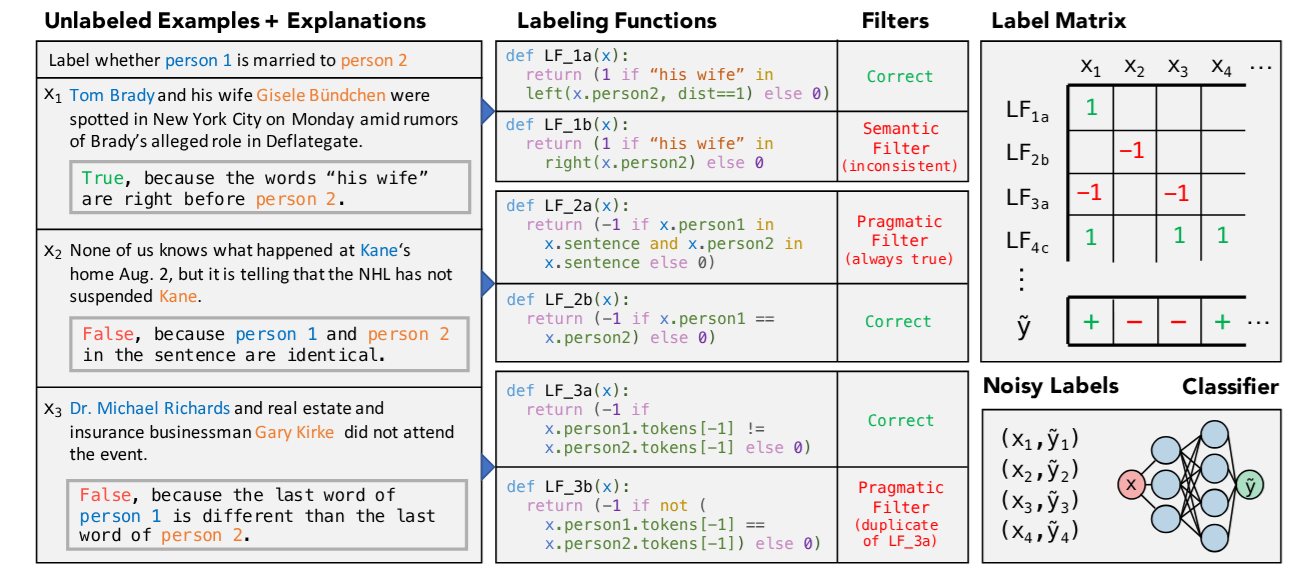
\includegraphics[keepaspectratio,alt={System Overview}]{fig-02.png}}
\caption{System Overview}
\end{figure}

}

\caption{\label{fig-02}Natural language explanations are parsed into
candidate labeling functions (LFs). Many incorrect LFs are filtered out
automatically by the filter bank. The remaining functions provide
heuristic labels over the unlabeled dataset, which are aggregated into
one noisy label per example, yielding a large, noisily-labeled training
set for a classifier.}

\end{marginfigure}%

\begin{marginfigure}

\centering{

\begin{figure}
\centering
\pandocbounded{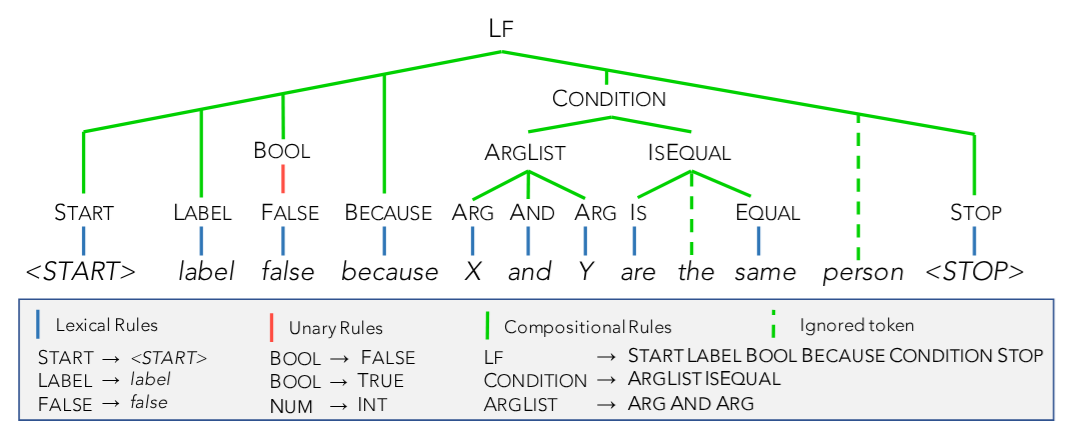
\includegraphics[keepaspectratio,alt={Seamntic Parse of An Explanation}]{fig-03.png}}
\caption{Seamntic Parse of An Explanation}
\end{figure}

}

\caption{\label{fig-03}Valid parses are found by iterating over
increasingly large sub-spans of the input looking for matches among the
right hand sides of the rules in the grammar. Rules are either lexical
(converting tokens into symbols), unary (converting one symbol into
another symbol), or compositional (combining many symbols into a single
higher-order symbol). A rule may optionally ignore unrecognized tokens
in a span (denoted here with a dashed line).}

\end{marginfigure}%

\subsubsection{Introduction}\label{introduction}

\begin{itemize}
\tightlist
\item
  Describes the standard protocol for collecting labeled data for
  training classifiers.
\item
  Highlights limitations of labeling: each label only provides a single
  bit of information.
\item
  Mentions previous works' approaches to improve information gain from
  examples.
\item
  Presents \texttt{BabbleLabble}, a framework where annotators provide
  natural language explanations for each labeling decision.
\end{itemize}

\subsubsection{\texorpdfstring{The \texttt{BabbleLabble}
Framework}{The BabbleLabble Framework}}\label{the-babblelabble-framework}

\begin{itemize}
\tightlist
\item
  Describes how \texttt{BabbleLabble} converts explanations and
  unlabeled data into a noisy training set.
\item
  Presents the three main components of \texttt{BabbleLabble}: semantic
  parser, filter bank, and label aggregator.
\item
  Mentions how explanations provide high-level information about
  patterns in the data.
\item
  Notes that the semantic parser converts explanations into a set of
  logical forms representing labeling functions.
\item
  Explains how the filter bank removes incorrect labeling functions
  based on semantic and pragmatic criteria.
\item
  Describes how the label aggregator combines labels from the labeling
  functions into probabilistic labels for each example.
\item
  Explains the benefits of training a discriminative model using the
  noisy labels instead of classifying directly with the label
  aggregator.
\end{itemize}

\subsubsection{Explanations}\label{explanations}

\begin{itemize}
\tightlist
\item
  Discusses the format and content of user-provided explanations.
\item
  Highlights that explanations should refer to specific aspects of the
  example.
\end{itemize}

\subsubsection{Semantic Parser}\label{semantic-parser}

\begin{itemize}
\tightlist
\item
  Describes the goal of the semantic parser: generate a set of candidate
  labeling functions (LFs).
\item
  Presents the rule-based semantic parser used in \texttt{BabbleLabble}
  and its key features.
\item
  Discusses the parser's grammar and the included predicates.
\item
  Notes that the parser is domain-independent, allowing transferability
  to new tasks.
\end{itemize}

\subsubsection{Filter Bank}\label{filter-bank}

\begin{itemize}
\tightlist
\item
  Explains the role of the filter bank: remove incorrect labeling
  functions without requiring ground truth labels.
\item
  Discusses the two types of filters: semantic and pragmatic.
\item
  Describes the purpose and operation of semantic and pragmatic filters.
\item
  Highlights the effectiveness of the filter bank in removing incorrect
  labeling functions.
\end{itemize}

\subsubsection{Label Aggregator}\label{label-aggregator}

\begin{itemize}
\tightlist
\item
  Explains the function of the label aggregator: combine potentially
  conflicting labels from multiple labeling functions into a single
  probabilistic label.
\item
  Discusses the limitations of a simple majority vote approach.
\item
  Presents the data programming approach used in \texttt{BabbleLabble},
  which models the relationship between true labels and labeling
  function outputs as a factor graph.
\end{itemize}

\subsubsection{Discriminative Model}\label{discriminative-model}

\begin{itemize}
\tightlist
\item
  Discusses the advantages of using a discriminative model trained with
  noisy labels.
\item
  Explains how a discriminative model can leverage features not
  explicitly mentioned in explanations.
\item
  Notes that the noisy labels provide a form of weak supervision that
  promotes generalization.
\end{itemize}

\subsubsection{Experimental Setup}\label{experimental-setup}

\begin{itemize}
\tightlist
\item
  Describes the three relation extraction tasks used for evaluation:
  Spouse, Disease, and Protein.
\item
  Presents details about each dataset: source, task description, and
  size.
\item
  Discusses the experimental settings: text preprocessing, semantic
  parser implementation, label aggregator, and discriminative model.
\item
  Mentions hyperparameter tuning and evaluation metrics.
\end{itemize}

\subsubsection{Experimental Results}\label{experimental-results}

\begin{itemize}
\tightlist
\item
  Presents the F1 scores achieved by \texttt{BabbleLabble} compared to
  traditional supervision.
\item
  Highlights the rate of improvement in F1 score with the number of user
  inputs.
\item
  Discusses the effectiveness of the filter bank in removing incorrect
  labeling functions.
\item
  Presents an analysis of the utility of incorrectly parsed labeling
  functions.
\item
  Compares using labeling functions as functions versus features.
\item
  Discusses the impact of unlabeled data on performance.
\end{itemize}

\subsubsection{Related Work and
Discussion}\label{related-work-and-discussion}

\begin{itemize}
\tightlist
\item
  Discusses previous work on learning from natural language
  explanations.
\item
  Mentions research on learning from weak supervision, particularly in
  the context of relation extraction.
\item
  Highlights the potential of natural language as a high-bandwidth
  communication channel for machine learning.
\item
  Discusses future research directions, including applying the framework
  to other tasks and exploring more interactive settings.
\end{itemize}

\begin{tcolorbox}[enhanced jigsaw, arc=.35mm, bottomrule=.15mm, bottomtitle=1mm, breakable, colback=white, colbacktitle=quarto-callout-caution-color!10!white, colframe=quarto-callout-caution-color-frame, coltitle=black, left=2mm, leftrule=.75mm, opacityback=0, opacitybacktitle=0.6, rightrule=.15mm, title=\textcolor{quarto-callout-caution-color}{\faFire}\hspace{0.5em}{My Thoughts}, titlerule=0mm, toprule=.15mm, toptitle=1mm]

\subsubsection{Big ideas}\label{big-ideas}

\begin{enumerate}
\def\labelenumi{\arabic{enumi}.}
\tightlist
\item
  \hl{Always be on the lookout for tricks on how to
  convert\footnotemark{} a supervised learning task into an unsupervised
  one}. While this paper fails to do so, it does provide a step in the
  right direction and more so one that yields a 100x speed up in
  labeling tasks. In reality this claim is a marketing shtick for their
  paper, however the real point is that if you have a labeling function,
  its utility grows in proportion to the amount of unlabeled data you
  can bring to bear.
\item
  Branden Hancock keeps reiterating that \hl{the bulk of the time spent
  in Labeling is understanding the text/data not the annotation}. The
  authors point that time to elicit explanation is only double the time
  of labeling. Highlighting evidence or even writing an explanation is
  thus a small burden in comparison to just annotating the most
  significant part of the text? Perhaps not yet if we include the
  benefits of the labeling functions that result in 6-10x more labels
  the math works out.
\item
  It is easy to miss the most significant aspect of the paper - \hl{the
  importance of the Filter Bank in creating value}. However there is an
  extensive literature on PBE (Program By Example) that they do not seem
  to be aware of which can convert such examples into programs.
\item
  Another point made by Branden in support of Explanation is that
  \hl{you can't highlight when the evidence is negative} - i.e.~when the
  classification is grounded in some context not being in the text.
\item
  A third reason to like explanations is that data-centric tasks are
  forever changing. There are new requirements (e.g.~a new class) or
  drifts in the classifiers's distributions. If you have collected
  labels you need to rethink the project but if you collected
  explanations it is easier to retain on more data then relabel. If
  there is a better semantic parser, you can swap it and re-train.
\end{enumerate}

\subsubsection{Devils and Details}\label{devils-and-details}

\begin{enumerate}
\def\labelenumi{\arabic{enumi}.}
\tightlist
\item
  The most interesting aspects of the paper for RL are how an agent
  interacting with people can elicit explanation that can then be used
  to create labeling functions.
\item
  The idea of how the labeling function are aggregated is also
  instructive. That said, I can't say that this is a big idea - it looks
  very much like ranking, weighting and even less powerful than TD-IDF.
  So what I mean is that when we learn a language probably want to learn
  features from functions not labels as labels do not generalize. If we
  also have a framing game that is driving language learning then we may
  have further uses for a sensible form of aggregation in our
  classifier. More abstractly, the RL agent needs to pick an action -
  that is usually like a classification of a state into an action space.
  For Life long learning we could
\item
  Q \& A are a good often considered in the Semantic Parsing literature.
\item
  LLM may well be useful for \hl{closing the weak supervision loop}.
  I.e. one can use a general purpose query to elicit explanations from
  an LLM. With a range of prompts one should be able to get different
  explanations.
\end{enumerate}

\subsubsection{Action Items}\label{action-items}

\begin{enumerate}
\def\labelenumi{\arabic{enumi}.}
\tightlist
\item
  Try babble labble, snorkel, prodigy, and SippyCup.
\item
  Make a MVP of the filter bank.
\item
  make a cheat-sheet on how to convert a supervised learning tasks into
  an unsupervised ones. These are ideas that disrupted the field of ML.
\item
  close the loop on weak supervision with LLM for a RL agent
\item
  compare this approach to other PBE
\end{enumerate}

\end{tcolorbox}

\footnotetext{TODO: make a cheat-sheet on this topic!?}

The people behind BabbleLabble are also behind Snorkel. Snorkel is a
framework for building weakly supervised models. It is a more general
framework that can be used for a wide range of tasks. BabbleLabble is a
specific application of Snorkel to the task of training classifiers with
natural language explanations. The key difference is that BabbleLabble
focuses on the use of natural language explanations to generate labeling
functions, while Snorkel is a more general framework for building weakly
supervised models.

A point made on the Snorkel Site is that the people who worked on the
tool moved on to building a platform. Is this just to monetize their
work? My guess is not. In reality there are many other tools that do
much the same thing. Labeling data is not very glamorous but building a
tool is just a ui and a classifier. You can't lock clients in and it is
likely that each project required expensive customization. At some point
it becomes simpler to do this in a form that is more general and can be
used by future clients. This is harder in open source as you need
consensus and a community. On the other hand in a platform each time you
do a project you have added value to the platform.

From other talks by Snorkel people it seems that many companies invest
massively in labeling datasets (i.e.~teams with sizes of hundreds). Thus
every small improvement in the process can have a big impact. And as a
business model it makes a lot of sense to try to bring as many of those
improvements in house.

\begin{tcolorbox}[enhanced jigsaw, arc=.35mm, bottomrule=.15mm, bottomtitle=1mm, breakable, colback=white, colbacktitle=quarto-callout-tip-color!10!white, colframe=quarto-callout-tip-color-frame, coltitle=black, left=2mm, leftrule=.75mm, opacityback=0, opacitybacktitle=0.6, rightrule=.15mm, title=\textcolor{quarto-callout-tip-color}{\faLightbulb}\hspace{0.5em}{Aggregation your'e No good for me}, titlerule=0mm, toprule=.15mm, toptitle=1mm]

Aggregation can take simple underlying components and combine them into
arbitrarily complex structures. This is a powerful idea that is used in
many areas of science and engineering. Here are a few examples:

\begin{enumerate}
\def\labelenumi{\arabic{enumi}.}
\item
  The Statistics the Central limit theorem allow us to aggregate many
  random variables into a Normal distributed one under fairly broad
  conditions.

  \begin{quote}
  ``Aggregate statistics can sometimes mask important information''. --
  Ben Bernanke
  \end{quote}
\item
  In Physics we can aggregate the behavior of many particles into that
  of an ensemble. We have a number of examples, the most famous being
  the ideal gas, statistical mechanics, the Ising model and the Potts
  model. Though the idea of aggregation is very much endemic to many
  areas of physics.

  \begin{quote}
  ``Imagine how difficult physics would be if electrons could think.''
  -- Murray Gell-Mann
  \end{quote}
\item
  In the case of a classifier we can aggregate many weak classifiers
  into a strong one. This is the idea behind \textbf{boosting} and
  \textbf{bagging}. This idea is behind well known algorithms like
  \textbf{Random Forest} and \textbf{Gradient Boosting} and even
  \textbf{Stable Diffusion}
\item
  In the case of a language we can aggregate the meaning or semantics of
  many smaller units of meaning into larger ones. This is the idea
  behind \textbf{semantics}. This idea is behind well known algorithms
  like \textbf{Word2Vec} and \textbf{BERT} and even \textbf{GPT-3}
\item
  Preferences can be aggregated into utility functions. This is the idea
  behind \textbf{utility theory}. This idea is behind demand theory.
\item
  Information aggregation is the notion that the wisdom of the crowd is
  better than the wisdom of the individual. \textbf{The Wisdom of the
  Crowds} points out that diverse opinions can play a big role here.
  There are other notions here like the \textbf{Delphi Method}.
\item
  Sensor Fusion via Kalman Filters, SLAM, and Particle Filters are ways
  to aggregate information from sensors. \textbf{The Kalman Filter} is a
  way to aggregate information from a sensor. \textbf{SLAM} is a way to
  aggregate information from a sensor. \textbf{Particle Filters} is a
  way to aggregate information from a sensor.
\item
  Social Networks have a number of ways to aggregate information.
  \textbf{PageRank} is a way to aggregate the importance of a node in a
  network. \textbf{The Small World Phenomenon} is a way to aggregate the
  number of hops between two nodes. \textbf{The Strength of Weak Ties}
  is a way to aggregate the number of connections between two nodes.
  \textbf{The Friendship Paradox} is a way to aggregate the number of
  friends a person has.
\item
  elections and voting have the notion of aggregation. \textbf{Arrow's
  Impossibility Theorem} points out that there is no perfect way to
  aggregate preferences. \textbf{The Condorcet Paradox} points out that
  there is no perfect way to aggregate opinions. \textbf{The
  Gibbard-Satterthwaite Theorem} points out that there is no perfect way
  to aggregate votes.
\item
  In chaos theory many chaotic systems can become synchronized.
\end{enumerate}

\end{tcolorbox}

\subsection{The Paper Annotated}\label{the-paper-annotated}

\begin{figure}[H]

{\centering 
\includegraphics[width=8.33333in,height=10.41667in]{paper.pdf}

}

\caption{paper}

\end{figure}%

\protect\phantomsection\label{refs}
\begin{CSLReferences}{1}{1}
\bibitem[\citeproctext]{ref-hancock2018trainingclassifiersnaturallanguage}
Hancock, Braden, Paroma Varma, Stephanie Wang, Martin Bringmann, Percy
Liang, and Christopher Ré. 2018. \emph{Training Classifiers with Natural
Language Explanations}. \url{https://arxiv.org/abs/1805.03818}.

\end{CSLReferences}




\end{document}
